Completa el crucigrama:
\begin{center}
    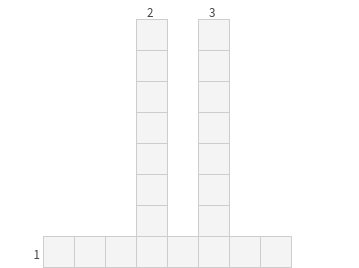
\includegraphics[width=0.5\textwidth]{Images/SINFI_U3_AC79_IMG1.png}
\end{center}

\begin{enumerate}
    \item Zona donde se conecta una neurona con otra.
    \item Permite el paso de iones positivos al interior y exterior de las neuronas en las células nerviosas.
    \item Células que se activan en la oscuridad o poca luz y perciben las intensidades luminosas entre el negro y el blanco.
\end{enumerate}